\documentclass[]{article}
\usepackage[left=1in,top=1in,right=1in,bottom=1in]{geometry}


%%%% more monte %%%%
% thispagestyle{empty}
% https://stackoverflow.com/questions/2166557/how-to-hide-the-page-number-in-latex-on-first-page-of-a-chapter
\usepackage{color}
% \usepackage[table]{xcolor} % are they using color?

% \definecolor{WSU.crimson}{HTML}{981e32}
% \definecolor{WSU.gray}{HTML}{5e6a71}

% \definecolor{shadecolor}{RGB}{248,248,248}
\definecolor{WSU.crimson}{RGB}{152,30,50} % use http://colors.mshaffer.com to convert from 981e32
\definecolor{WSU.gray}{RGB}{94,106,113}

%%%%%%%%%%%%%%%%%%%%%%%%%%%%

\newcommand*{\authorfont}{\fontfamily{phv}\selectfont}
\usepackage{lmodern}


  \usepackage[T1]{fontenc}
  \usepackage[utf8]{inputenc}




\usepackage{abstract}
\renewcommand{\abstractname}{}    % clear the title
\renewcommand{\absnamepos}{empty} % originally center

\renewenvironment{abstract}
 {{%
    \setlength{\leftmargin}{0mm}
    \setlength{\rightmargin}{\leftmargin}%
  }%
  \relax}
 {\endlist}

\makeatletter
\def\@maketitle{%
  \pagestyle{empty}
  \newpage
%  \null
%  \vskip 2em%
%  \begin{center}%
  \let \footnote \thanks
    {\fontsize{18}{20}\selectfont\raggedright  \setlength{\parindent}{0pt} \@title \par}%
}
%\fi
\makeatother






\usepackage{color}
\usepackage{fancyvrb}
\newcommand{\VerbBar}{|}
\newcommand{\VERB}{\Verb[commandchars=\\\{\}]}
\DefineVerbatimEnvironment{Highlighting}{Verbatim}{commandchars=\\\{\}}
% Add ',fontsize=\small' for more characters per line
\usepackage{framed}
\definecolor{shadecolor}{RGB}{248,248,248}
\newenvironment{Shaded}{\begin{snugshade}}{\end{snugshade}}
\newcommand{\AlertTok}[1]{\textcolor[rgb]{0.94,0.16,0.16}{#1}}
\newcommand{\AnnotationTok}[1]{\textcolor[rgb]{0.56,0.35,0.01}{\textbf{\textit{#1}}}}
\newcommand{\AttributeTok}[1]{\textcolor[rgb]{0.77,0.63,0.00}{#1}}
\newcommand{\BaseNTok}[1]{\textcolor[rgb]{0.00,0.00,0.81}{#1}}
\newcommand{\BuiltInTok}[1]{#1}
\newcommand{\CharTok}[1]{\textcolor[rgb]{0.31,0.60,0.02}{#1}}
\newcommand{\CommentTok}[1]{\textcolor[rgb]{0.56,0.35,0.01}{\textit{#1}}}
\newcommand{\CommentVarTok}[1]{\textcolor[rgb]{0.56,0.35,0.01}{\textbf{\textit{#1}}}}
\newcommand{\ConstantTok}[1]{\textcolor[rgb]{0.00,0.00,0.00}{#1}}
\newcommand{\ControlFlowTok}[1]{\textcolor[rgb]{0.13,0.29,0.53}{\textbf{#1}}}
\newcommand{\DataTypeTok}[1]{\textcolor[rgb]{0.13,0.29,0.53}{#1}}
\newcommand{\DecValTok}[1]{\textcolor[rgb]{0.00,0.00,0.81}{#1}}
\newcommand{\DocumentationTok}[1]{\textcolor[rgb]{0.56,0.35,0.01}{\textbf{\textit{#1}}}}
\newcommand{\ErrorTok}[1]{\textcolor[rgb]{0.64,0.00,0.00}{\textbf{#1}}}
\newcommand{\ExtensionTok}[1]{#1}
\newcommand{\FloatTok}[1]{\textcolor[rgb]{0.00,0.00,0.81}{#1}}
\newcommand{\FunctionTok}[1]{\textcolor[rgb]{0.00,0.00,0.00}{#1}}
\newcommand{\ImportTok}[1]{#1}
\newcommand{\InformationTok}[1]{\textcolor[rgb]{0.56,0.35,0.01}{\textbf{\textit{#1}}}}
\newcommand{\KeywordTok}[1]{\textcolor[rgb]{0.13,0.29,0.53}{\textbf{#1}}}
\newcommand{\NormalTok}[1]{#1}
\newcommand{\OperatorTok}[1]{\textcolor[rgb]{0.81,0.36,0.00}{\textbf{#1}}}
\newcommand{\OtherTok}[1]{\textcolor[rgb]{0.56,0.35,0.01}{#1}}
\newcommand{\PreprocessorTok}[1]{\textcolor[rgb]{0.56,0.35,0.01}{\textit{#1}}}
\newcommand{\RegionMarkerTok}[1]{#1}
\newcommand{\SpecialCharTok}[1]{\textcolor[rgb]{0.00,0.00,0.00}{#1}}
\newcommand{\SpecialStringTok}[1]{\textcolor[rgb]{0.31,0.60,0.02}{#1}}
\newcommand{\StringTok}[1]{\textcolor[rgb]{0.31,0.60,0.02}{#1}}
\newcommand{\VariableTok}[1]{\textcolor[rgb]{0.00,0.00,0.00}{#1}}
\newcommand{\VerbatimStringTok}[1]{\textcolor[rgb]{0.31,0.60,0.02}{#1}}
\newcommand{\WarningTok}[1]{\textcolor[rgb]{0.56,0.35,0.01}{\textbf{\textit{#1}}}}



\title{\textbf{\textcolor{WSU.crimson}{The Modern Vitruvian
Man}} \newline \textbf{\textcolor{WSU.gray}{Body Proportions}}  }
 

%  

% \author{ \Large true \hfill \normalsize \emph{} }
\author{\Large Nathan
Shine\vspace{0.05in} \newline\normalsize\emph{Washington State
University}  }


\date{November 08, 2020}
\setcounter{secnumdepth}{3}

\usepackage{titlesec}
% See the link above: KOMA classes are not compatible with titlesec any more. Sorry.
% https://github.com/jbezos/titlesec/issues/11
\titleformat*{\section}{\bfseries}
\titleformat*{\subsection}{\bfseries\itshape}
\titleformat*{\subsubsection}{\itshape}
\titleformat*{\paragraph}{\itshape}
\titleformat*{\subparagraph}{\itshape}

% https://code.usgs.gov/usgs/norock/irvine_k/ip-092225/


%\titleformat*{\section}{\normalsize\bfseries}
%\titleformat*{\subsection}{\normalsize\itshape}
%\titleformat*{\subsubsection}{\normalsize\itshape}
%\titleformat*{\paragraph}{\normalsize\itshape}
%\titleformat*{\subparagraph}{\normalsize\itshape}

% https://tex.stackexchange.com/questions/233866/one-column-multicol-environment#233904
\usepackage{environ}
\NewEnviron{auxmulticols}[1]{%
  \ifnum#1<2\relax% Fewer than 2 columns
    %\vspace{-\baselineskip}% Possible vertical correction
    \BODY
  \else% More than 1 column
    \begin{multicols}{#1}
      \BODY
    \end{multicols}%
  \fi
}





\usepackage{natbib}
\setcitestyle{aysep={}} %% no year, comma just year
% \usepackage[numbers]{natbib}
\bibliographystyle{./../biblio/ormsv080.bst}



\usepackage[strings]{underscore} % protect underscores in most circumstances




\newtheorem{hypothesis}{Hypothesis}
\usepackage{setspace}


%%%%%%%%%%%%%%%%%%%%%%%%%%%%%%%%%%%%%%%%%%%%%%%%%%%%%
%%% MONTE ADDS %%%

\usepackage{fancyhdr} % fancy header 
\usepackage{lastpage} % last page 

\usepackage{multicol}


\usepackage{etoolbox}
\AtBeginEnvironment{quote}{\singlespacing\small}
% https://tex.stackexchange.com/questions/325695/how-to-style-blockquote


\usepackage{soul}			%% allows strike-through
\usepackage{url}			%% fixes underscores in urls
\usepackage{csquotes}		%% allows \textquote in references
\usepackage{rotating}		%% allows table and box rotation
\usepackage{caption}		%% customize caption information
\usepackage{booktabs}		%% enhance table/tabular environment
\usepackage{tabularx}		%% width attributes updates tabular
\usepackage{enumerate}		%% special item environment
\usepackage{enumitem}		%% special item environment

\usepackage{lineno}		%% allows linenumbers for editing using \linenumbers
\usepackage{hanging}


\usepackage{mathtools}  	%% also loads amsmath
\usepackage{bm}		%% bold-math
\usepackage{scalerel}	%% scale one element (make one beta bigger font)

\newcommand{\gFrac}[2]{ \genfrac{}{}{0pt}{1}{{#1}}{#2} }

\newcommand{\betaSH}[3]{  \gFrac{\text{\tiny #1}}{{\text{\tiny #2}}}\hat{\beta}_{\text{#3}}   }
\newcommand{\betaSB}[3]{              ^{\text{#1}} _{\text{#2}} \bm{\beta} _{\text{#3}}                   }  %% bold
\newcommand{\bigEQ}{  \scaleobj{1.5}{{\ }= } }
\newcommand{\bigP}[1]{  \scaleobj{1.5}{#1 } }





\usepackage{endnotes}  % he already does this ...
\renewcommand{\enotesize}{\normalsize}
% https://tex.stackexchange.com/questions/99984/endnotes-do-not-be-superscript-and-add-a-space
\renewcommand\makeenmark{\textsuperscript{[\theenmark]}} % in brackets %
% https://tex.stackexchange.com/questions/31574/how-to-control-the-indent-in-endnotes
\patchcmd{\enoteformat}{1.8em}{0pt}{}{}

\patchcmd{\theendnotes}
  {\makeatletter}
  {\makeatletter\renewcommand\makeenmark{\textbf{[\theenmark]} }}
  {}{}



% https://tex.stackexchange.com/questions/141906/configuring-footnote-position-and-spacing

\addtolength{\footnotesep}{5mm} % change to 1mm

\renewcommand{\thefootnote}{\textbf{\arabic{footnote}}}
\let\footnote=\endnote
%\renewcommand*{\theendnote}{\alph{endnote}}
%\renewcommand{\theendnote}{\textbf{\arabic{endnote}}}


\renewcommand*{\notesname}{ENDNOTES}

\makeatletter
\def\enoteheading{\section*{\notesname
  \@mkboth{\MakeUppercase{\notesname}}{\MakeUppercase{\notesname}}}%
  \mbox{}\par\vskip-2.3\baselineskip\noindent\rule{.5\textwidth}{0.4pt}\par\vskip\baselineskip}
\makeatother


\renewcommand*{\contentsname}{TABLE OF CONTENTS}

\renewcommand*{\refname}{REFERENCES}


%\usepackage{subfigure}
\usepackage{subcaption}

\captionsetup{labelfont=bf}  % Make Table / Figure bold

%%% you could add elements here ... monte says .... %%%
%\usepackage{mypackageForCapitalH}


%%%%%%%%%%%%%%%%%%%%%%%%%%%%%%%%%%%%%%%%%%%%%%%%%%%%%

% set default figure placement to htbp
\makeatletter
\def\fps@figure{htbp}
\makeatother


% move the hyperref stuff down here, after header-includes, to allow for - \usepackage{hyperref}

\makeatletter
\@ifpackageloaded{hyperref}{}{%
\ifxetex
  \PassOptionsToPackage{hyphens}{url}\usepackage[setpagesize=false, % page size defined by xetex
              unicode=false, % unicode breaks when used with xetex
              xetex]{hyperref}
\else
  \PassOptionsToPackage{hyphens}{url}\usepackage[draft,unicode=true]{hyperref}
\fi
}

\@ifpackageloaded{color}{
    \PassOptionsToPackage{usenames,dvipsnames}{color}
}{%
    \usepackage[usenames,dvipsnames]{color}
}
\makeatother
\hypersetup{breaklinks=true,
            bookmarks=true,
            pdfauthor={Nathan Shine (Washington State University)},
             pdfkeywords = {multiple comparisons to control;
multivariate chi-square distribution; nonlinear growth curves; Richard's
curve; simulated critical points},  
            pdftitle={The Modern Vitruvian Man: Body Proportions},
            colorlinks=true,
            citecolor=blue,
            urlcolor=blue,
            linkcolor=magenta,
            pdfborder={0 0 0}}
\urlstyle{same}  % don't use monospace font for urls

% Add an option for endnotes. -----

%
% add tightlist ----------
\providecommand{\tightlist}{%
\setlength{\itemsep}{0pt}\setlength{\parskip}{0pt}}

% add some other packages ----------

% \usepackage{multicol}
% This should regulate where figures float
% See: https://tex.stackexchange.com/questions/2275/keeping-tables-figures-close-to-where-they-are-mentioned
\usepackage[section]{placeins}



\pagestyle{fancy}   
\lhead{\textcolor{WSU.crimson}{\textbf{ The Modern Vitruvian Man }}}
\chead{}
\rhead{\textcolor{WSU.gray}{\textbf{  Page\ \thepage\ of\ \protect\pageref{LastPage} }}}
\lfoot{}
\cfoot{}
\rfoot{}


\begin{document}
	
% \pagenumbering{arabic}% resets `page` counter to 1 
%    

% \maketitle

{% \usefont{T1}{pnc}{m}{n}
\setlength{\parindent}{0pt}
\thispagestyle{plain}
{\fontsize{18}{20}\selectfont\raggedright 
\maketitle  % title \par  

}

{
   \vskip 13.5pt\relax \normalsize\fontsize{11}{12} 
   
\textbf{\authorfont Nathan Shine} \hskip 15pt \emph{\small Washington
State University}   

}

}








\begin{abstract}

    \hbox{\vrule height .2pt width 39.14pc}

    \vskip 8.5pt % \small 

\noindent In this article we compare the
\emph{empirical characteristic function} \citep{Tukey:1977, Becker:1988}
to a \emph{moment-generating-functional form} to compute the proportion
of hypotheses \(m\) that are rejected under the null hypothesis.
\vspace{0.25in}

\noindent Here is a second paragraph of the abstract (if necessary), and
with the pipe notation it doesn't break. Notice it still needs to be
indented. \vspace{0.25in}

\noindent Generally, we write this abstract last. Often it is called the
executive summary. It should succinctly summarize the entire document.
You can include references such as this one to the Appendices section
\ref{sec:appendix} if necessary.


\vskip 8.5pt \noindent \textbf{\underline{Keywords}:} multiple
comparisons to control; multivariate chi-square distribution; nonlinear
growth curves; Richard's curve; simulated critical points \par

    




    
    \hbox{\vrule height .2pt width 39.14pc}
    \vskip 5pt 
    \hfill \textbf{\textcolor{WSU.gray}{ November 08, 2020 } }
    \vskip 5pt 
    
\end{abstract}


\vskip -8.5pt



 % removetitleabstract

\noindent  

\section{Introduction}
\label{sec:intro}

Write something here.

{[}ONE GRAPHIC{]}

{[}TWO GRAPHICS AS ONE{]}

Write something here.

\section{Research Question:  Are the Vitruvian Man proportions realistic? How likely are men to be close to these proportions?}
\label{sec:rq}

The Vitruvian Man was designed with certain proportions in mind.
Vitruvius was a Roman architect and in his writings he describes the
human body as a set of proportions of one's height. \newline

\begin{quote}
"the open hand from the wrist to the tip of the middle finger is [a tenth part of the whole height]; the head from the chin to the crown is an eighth, ... The length of the foot is one sixth of the height of the body... and the breadth of the breast is also one fourth... outstretched arms... will be found to be the same as the height"
\end{quote}

\citep{Vitruvius} \newline

\begin{center}
\begin{tabular}{ l c}
  \label{tab:vitruvian-props}
  \textbf{Body length} & \textbf{Vitruvian Man proportions}\\
  \hline
  Head height & 0.125\\
  Arm span & 1.000\\
  Hand length & 0.100\\
  Foot length & 0.167\\
  Knee height & 0.250\\
  Shoulder width & 0.250\\
\end{tabular}
\end{center}
\subsection{Does height affect the body proportions for men and women?}
\label{sec:rq2}

\subsection{What body proportions for men and women are realistic today?}
\label{sec:rq3}

\section{Data Description}
\label{sec:data}

The data was collected by approximately 30 students who are enrolled in
STAT 419 at WSU. Students were supposed to gather measurements from at
least ten people. The measurements gathered were: height, head height,
head circumference, arm span, floor to navel, hand length, hand width,
hand to elbow, elbow to armpit, arm reach, foot length, floor to
knee-pit, floor to hip, and floor to armpit. The measurements were
collected by having either the student or another measure the subject
with a measuring tape such as the ones used by tailors. Students were
also asked to record which side of the body the measurements came from.
Some students chose to gather measurements from both sides for the sake
of completeness.

The data from all students was then compiled into one dataset. The total
dataset contains 263 rows of measurements. Covariates for each row were
also collected. Each subject was instructed to identify their writing
hand, swinging hand, dominant eye, eye color, age, gender, and
ethnicity. The data collector then assigned a value (1-10) assessing the
quality of the measurements taken, and recorded the amount of minutes
that it took to complete the measurements.

\subsection{Summary of Sample}
\label{sec:data-sample}

The sample contained about equal parts male and female subjects.
Subjects identifying as white made up about 70\% of the dataset, the
next largest ethnicity was Asian, which contained about 15\% of
subjects. The majority of those sampled were in their 20s. There were
not many under 10 or over 70 sampled. Subjects who preferred their
right-side made up about 80\% of the sample. Most subjects had brown or
blue eyes --46 and 31 percent respectively-- with a a lesser number of
hazel or green eyed persons. The quality of the data collected ranged
mostly between 8-10 on a 10-point scale. Most data collectors took
between 10-20 minutes to gather all measurements required.

\begin{figure}[!ht]
    \begin{subfigure}[h]{0.5\textwidth}
    \centering
    %  trim={<left> <lower> <right> <upper>}
    % https://shantoroy.com/latex/add-subfig-in-latex/
            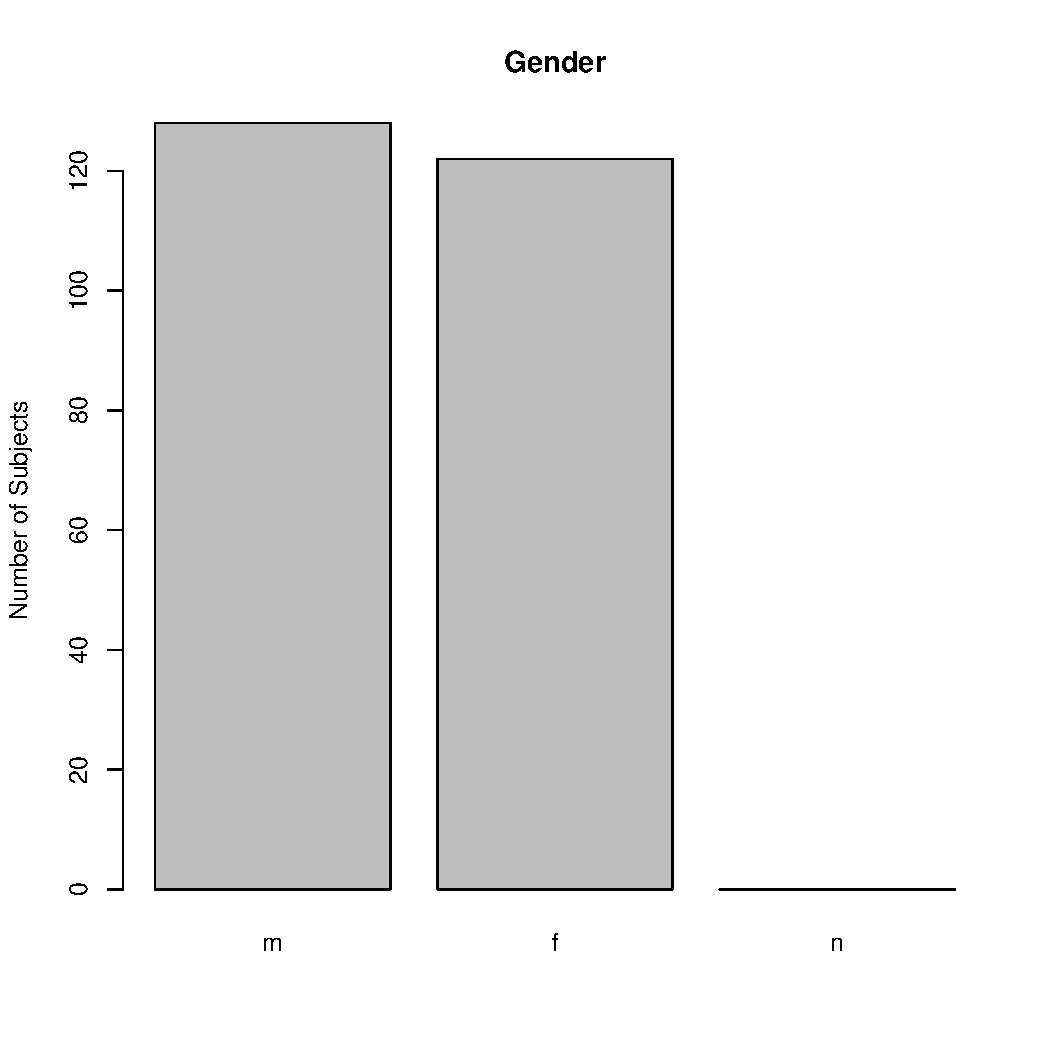
\includegraphics[clip,scale=0.4]{figures/gender-plot.pdf}
        \caption{ Gender Distribution}
        \label{fig:gender-plot}
    \end{subfigure}
    \begin{subfigure}[h]{0.5\textwidth}
    \centering
        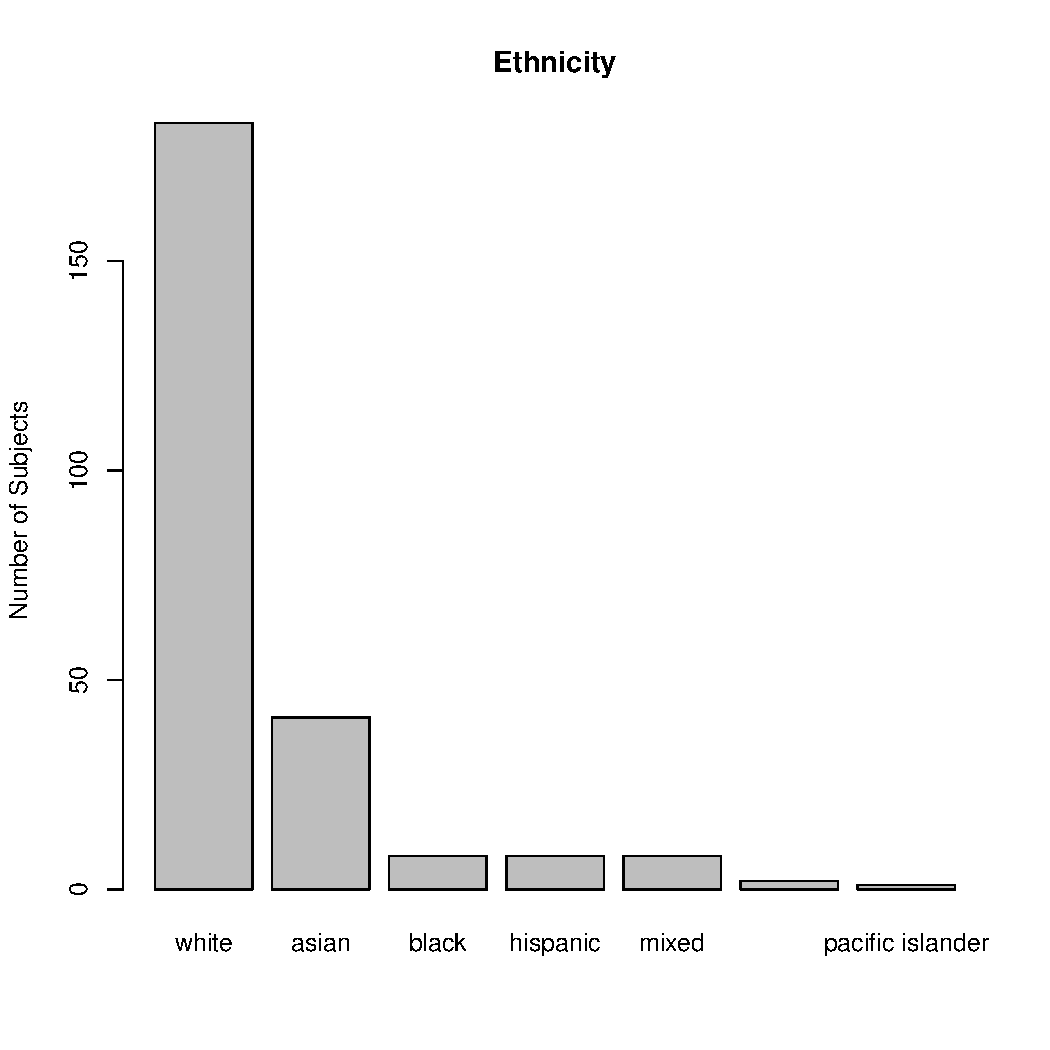
\includegraphics[clip,scale=0.4]{figures/ethnicity-plot.pdf}
            \caption{Ethnicity Distribution}
        \label{fig:ethnicity-plot}
    \end{subfigure}
    \vspace{2.5mm}
    \hrule
    \vspace{2.5mm}
        \caption{\textbf{ Gender and Ethnicity Distributions } }
        \label{fig:ge-plot}
\end{figure}

\newpage
\subsection{Summary Statistics of Data}
\label{sec:data-summary}

By comparing tables below we can see that the average proportion for
both male and female subjects are about the same. However, the standard
deviations show that males vary more in arm span and shoulder width. To
a lesser extent males vary more with hand length as well. Females have a
more variable head.height proportion. Females also have a slightly more
variable foot length and floor to knee-pit length.

\begin{table}[!htbp]
\footnotesize
\centering
\caption{\textbf{Descriptive Statistics and Correlation Analysis (FEMALE)}}
\label{table:correlation-female}
\begin{tabularx}{1\textwidth}{{r@{ \ \ } p{30mm} r@{}lp{1mm} r@{}l p{5mm} r@{}l p{2mm} r@{}l p{2mm} r@{}l p{2mm} r@{}l p{2mm} r@{}l p{2mm}   r@{}l  }}
 & \\
\hline
 & \\
\multicolumn{2}{c}{\textbf{ }} & \multicolumn{2}{c}{\textbf{M}} & & \multicolumn{2}{c}{\textbf{SD}} &  & \multicolumn{2}{c}{\textbf{1}} &  & \multicolumn{2}{c}{\textbf{2}} &  & \multicolumn{2}{c}{\textbf{3}} &  & \multicolumn{2}{c}{\textbf{4}} &  & \multicolumn{2}{c}{\textbf{5}} &  & \\ 
 & \\
\hline
 & \\
\textbf{1} & \textbf{head.height} &  &.133 &  &  &.017 &  &  1&  &  &  \multicolumn{2}{c}{ \  \  \  \  \ }  &  &  \multicolumn{2}{c}{ \  \  \  \  \ }  &  &  \multicolumn{2}{c}{ \  \  \  \  \ }  &  &  \multicolumn{2}{c}{ \  \  \  \  \ }  &  & \\ 
 & \\
\textbf{2} & \textbf{arm.span} &  1&.008 &  &  &.050 &  &  -&.04 &  &  1&  &  &  \multicolumn{2}{c}{ \  \  \  \  \ }  &  &  \multicolumn{2}{c}{ \  \  \  \  \ }  &  &  \multicolumn{2}{c}{ \  \  \  \  \ }  &  & \\ 
 & \\
\textbf{3} & \textbf{hand.length} &  &.108 &  &  &.007 &  &  &.30{$^{**}$}  &  &  &.03 &  &  1&  &  &  \multicolumn{2}{c}{ \  \  \  \  \ }  &  &  \multicolumn{2}{c}{ \  \  \  \  \ }  &  & \\ 
 & \\
\textbf{4} & \textbf{foot.length} &  &.145 &  &  &.010 &  &  &.22{$^{*}$}  &  &  &.18{$^{\dagger}$}  &  &  &.48{$^{***}$}  &  &  1&  &  &  \multicolumn{2}{c}{ \  \  \  \  \ }  &  & \\ 
 & \\
\textbf{5} & \textbf{floor.kneepit} &  &.267 &  &  &.019 &  &  &.12 &  &  &.06 &  &  &.29{$^{**}$}  &  &  &.30{$^{**}$}  &  &  1&  &  & \\ 
 & \\
\textbf{6} & \textbf{shoulder.width} &  &.186 &  &  &.065 &  &  &.01 &  &  &.55{$^{***}$}  &  &  -&.06 &  &  -&.04 &  &  -&.10 &  & \\ 
 & \\
\hline
 & \\
\multicolumn{22}{p{0.9\textwidth}}{  \footnotesize { \begin{hangparas}{0.75in}{1} \textbf{\underline{Notes}:} \ \ Pearson pairwise correlations are reported; \newline a two-side test was performed to report correlation significance.  \end{hangparas} } }  & \\  
\multicolumn{22}{p{0.9\textwidth}}{  {\tiny {$^{\dagger} p < .10$} }  {     } {\tiny        {$^{*} p < .05$} }  {     } {\tiny       {$^{**} p < .01$} }  {     } {\tiny      {$^{***} p < .001$} } {     }     } & \\ 
 & \\
\hline
\end{tabularx}
\end{table}

\begin{table}[!htbp]
\footnotesize
\centering
\caption{\textbf{Descriptive Statistics and Correlation Analysis (MALE)}}
\label{table:correlation-male}
\begin{tabularx}{1\textwidth}{{r@{ \ \ } p{30mm} r@{}lp{1mm} r@{}l p{5mm} r@{}l p{2mm} r@{}l p{2mm} r@{}l p{2mm} r@{}l p{2mm} r@{}l p{2mm}   r@{}l  }}
 & \\
\hline
 & \\
\multicolumn{2}{c}{\textbf{ }} & \multicolumn{2}{c}{\textbf{M}} & & \multicolumn{2}{c}{\textbf{SD}} &  & \multicolumn{2}{c}{\textbf{1}} &  & \multicolumn{2}{c}{\textbf{2}} &  & \multicolumn{2}{c}{\textbf{3}} &  & \multicolumn{2}{c}{\textbf{4}} &  & \multicolumn{2}{c}{\textbf{5}} &  & \\ 
 & \\
\hline
 & \\
\textbf{1} & \textbf{head.height} &  &.130 &  &  &.013 &  &  1&  &  &  \multicolumn{2}{c}{ \  \  \  \  \ }  &  &  \multicolumn{2}{c}{ \  \  \  \  \ }  &  &  \multicolumn{2}{c}{ \  \  \  \  \ }  &  &  \multicolumn{2}{c}{ \  \  \  \  \ }  &  & \\ 
 & \\
\textbf{2} & \textbf{arm.span} &  1&.011 &  &  &.062 &  &  -&.28{$^{**}$}  &  &  1&  &  &  \multicolumn{2}{c}{ \  \  \  \  \ }  &  &  \multicolumn{2}{c}{ \  \  \  \  \ }  &  &  \multicolumn{2}{c}{ \  \  \  \  \ }  &  & \\ 
 & \\
\textbf{3} & \textbf{hand.length} &  &.109 &  &  &.008 &  &  &.36{$^{***}$}  &  &  -&.09 &  &  1&  &  &  \multicolumn{2}{c}{ \  \  \  \  \ }  &  &  \multicolumn{2}{c}{ \  \  \  \  \ }  &  & \\ 
 & \\
\textbf{4} & \textbf{foot.length} &  &.148 &  &  &.009 &  &  &.14 &  &  -&.07 &  &  &.52{$^{***}$}  &  &  1&  &  &  \multicolumn{2}{c}{ \  \  \  \  \ }  &  & \\ 
 & \\
\textbf{5} & \textbf{floor.kneepit} &  &.267 &  &  &.018 &  &  &.26{$^{**}$}  &  &  -&.20{$^{*}$}  &  &  &.05 &  &  &.16{$^{\dagger}$}  &  &  1&  &  & \\ 
 & \\
\textbf{6} & \textbf{shoulder.width} &  &.203 &  &  &.092 &  &  -&.14 &  &  &.55{$^{***}$}  &  &  -&.16 &  &  -&.15 &  &  -&.08 &  & \\ 
 & \\
\hline
 & \\
\multicolumn{22}{p{0.9\textwidth}}{  \footnotesize { \begin{hangparas}{0.75in}{1} \textbf{\underline{Notes}:} \ \ Pearson pairwise correlations are reported; \newline a two-side test was performed to report correlation significance.  \end{hangparas} } }  & \\  
\multicolumn{22}{p{0.9\textwidth}}{  {\tiny {$^{\dagger} p < .10$} }  {     } {\tiny        {$^{*} p < .05$} }  {     } {\tiny       {$^{**} p < .01$} }  {     } {\tiny      {$^{***} p < .001$} } {     }     } & \\ 
 & \\
\hline
\end{tabularx}
\end{table}


Male and female subjects have the significant positive correlations for
hand length and head height, shoulder width and arm span, and foot
length and hand length. This means that for any person if they have
wider shoulders, then they are likely to have a bigger arm span. If a
person has longer hands they are more likely to have a taller head and
longer feet. For male subjects there is also a negative correlation
between arm span and head height, meaning that those with bigger arm
spans are likely to have shorter heads. However, there is a positive
correlation for males between the height of the knee and the height of
the head, meaning that a male with a higher knee (or longer legs?) is
more likely to have a longer head. For female subjects there are
significant positive correlations between the height of the knee, and
both hand length and foot length. This suggests that females with longer
legs may have longer feet and hands.

\newpage

\section{Key Findings}
\label{sec:findings}

\section{Conclusion}
\label{sec:conclusion}

\newpage

This was a new page

This is a newline. \newline  Here is some more text.

Below are some example code that may benefit you in preparing your
document. \newline

\vspace{0.25in}

\noindent Please state your name: \hrulefill \newline I was born on
\hrulefill in \hrulefill \vspace{0.25in}

\begin{equation}
\label{eq:my-model}
    Y_{jt} = \alpha + \bm{\beta}X_{jt} + \upsilon_{j}  + \varepsilon_{jt} ,
\end{equation}

\noindent where \(\alpha\) is the grand mean, \(\upsilon_{j}\) is the
fixed-time country mean, \(X_{jt}\) (country \(j\) at time \(t\)) is the
matrix of country-level observations for the vector of aforementioned
parameters \(\bm{\beta}\), and \(\varepsilon_{jt}\) represents the
residual idiosyncratic disturbance. Our panel data set consists of
repeated observations of countries over time. Therefore, we employ
cross-section time-series models. This approach redefines
Equation\textasciitilde{}\ref{eq:my-model} by subtracting time-demeaned
values. This \emph{within} transformation subtracts constant country
effects for the dependent variable \(\bar{Y_{j}}\), the predictor
variables \(\bar{X_{j}}\), and the intercept \(\bar{\upsilon_{j}}\):

\begin{equation}
\label{eq:my-random}
    (Y_{jt} - \theta \bar{Y_{j}}) = (1-\theta)\alpha + \bm{\beta}(X_{jt} - \bar{X_{j}}) +  (\upsilon_{jt} - \theta \bar{\upsilon_{j}})  ,
\end{equation}

\noindent If \(\theta = 0\), the model reduces to a basic pooled
ordinary-least-squares (OLS) model; if \(\theta = 1\), the model reduces
to a fixed-effects model; otherwise the model represents a
random-effects model. The pooled OLS estimation is biased if country
effects exist \citep{Hsiao:2003}. The random-effects model may be
susceptible to omitted-variable bias \citep{Wooldridge:2006}: bias
because a predictor was excluded from the model specification.
Conversely, the fixed-effects model is not susceptible to this bias as
it captures unobserved intracountry variation around its average
country-level ``fixed effect." Panel-data analysis commonly has issues
with heteroskedasticity, serial autocorrelation, and cross-sectional
autocorrelation.

\vspace{0.5in}

\(i=1\) and \[i = 1\]

\vspace{0.5in}

\begin{tabular}{ c c c c c}
  1 & 2 & 3 & 4 & 5 \\
  \hline
  6 & 7 & 8 & 9 & 10
\end{tabular}

\vspace{0.5in}

\begin{figure}[!ht]
%% figures have hrule, tables have hline
    \hrule
    \caption{ \textbf{Conceptual Model} }
    \begin{center}
        \scalebox{1.00}{    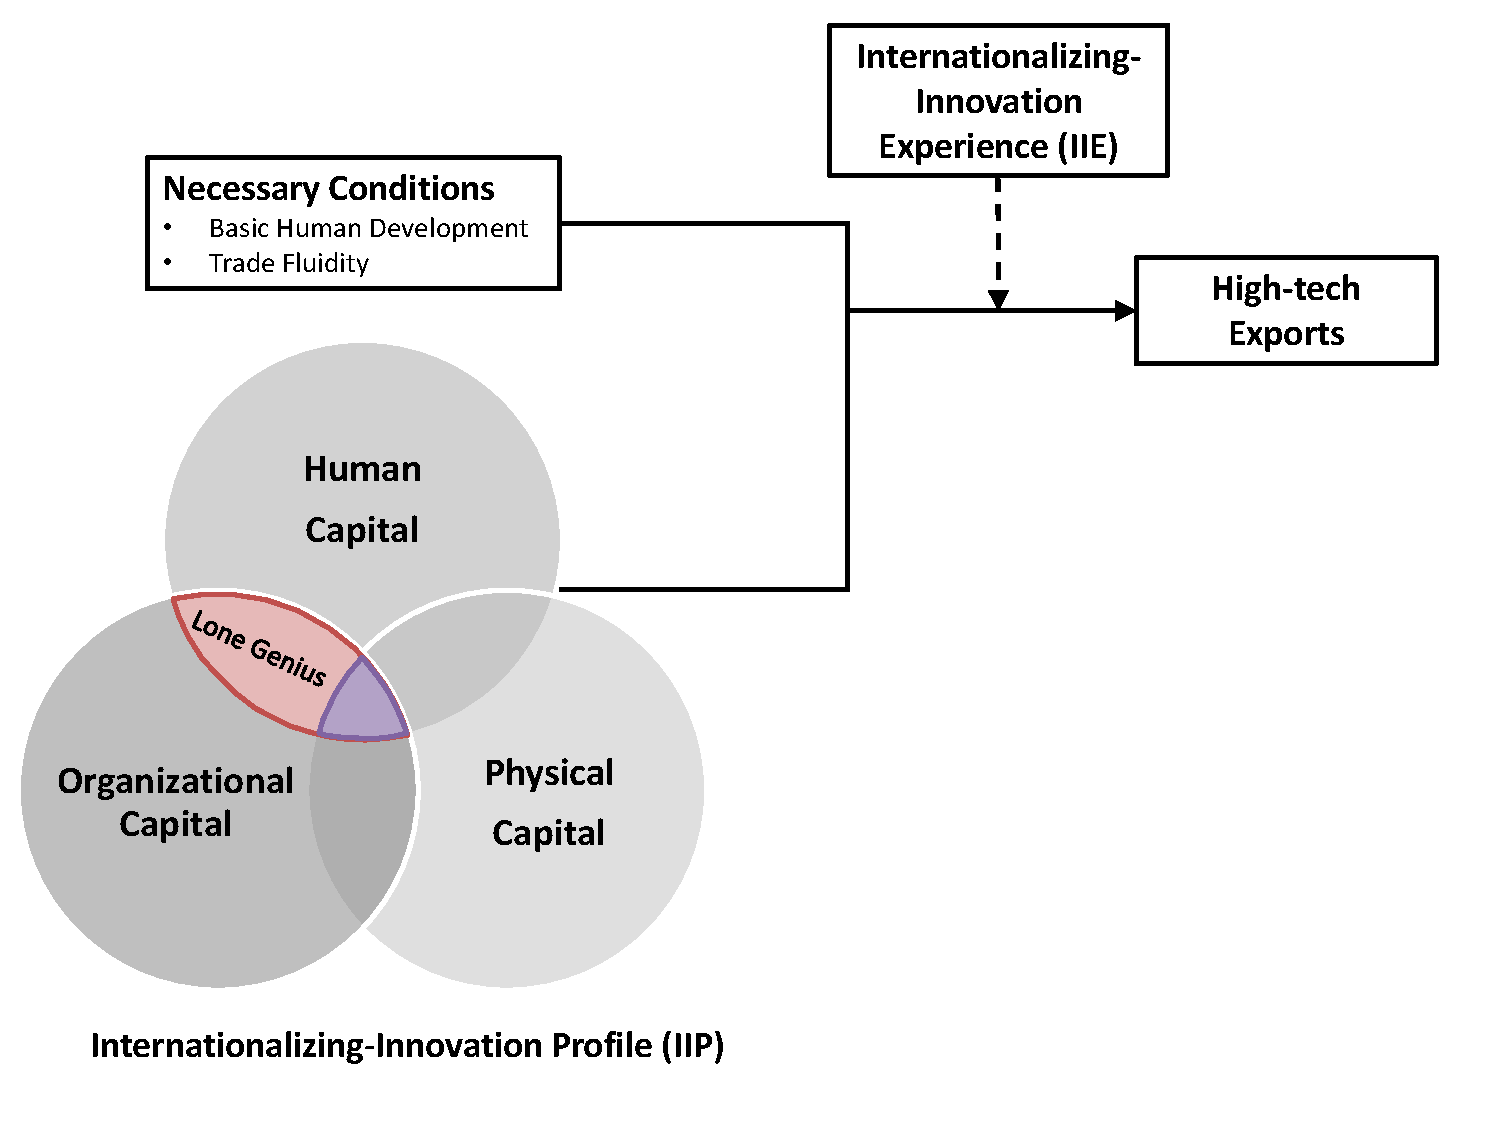
\includegraphics[trim = 0 0 0 0,clip,width=\textwidth]{figures/conceptual-model-v4.pdf} }
    \end{center}
    \label{fig:conceptual-model}
    \hrule
\end{figure}

See Figure \ref{fig:conceptual-model}.

\newpage

This is a
footnote\footnote{This is a footnote that can be really long.  \newline You can have multiple paragraphs in the footnote.  You can have \underline{underline} or \textbf{bold} or \emph{italics}.  You can even have a math equation inline. \newline In this section, we review the regression results to summarize our findings.  First, we examine each model for significance, and conclude the hypothesized models fit well with the data.  Second, we conclude that the fixed country effects represent consistent and unbiased parameter estimates.  Third, with the use of the \citet{Driscoll:1998} robust standard errors, we adjust any variance bias to ascertain the significance of these consistent estimates.  Therefore, we are able to make inferences about the hypotheses using our model estimates.  For ease of interpretation across these 12 models, we introduce $\betaSH{{ \ \ }M1}{Total}{1}$ as notation to refer to parameter estimate $\hat{\beta}_{1}$ (HDI) for the Total Sample and (M1) Model 1:  Main Effects.  We proceed by reporting findings for the total sample. \newline The footnotes are automatically converted to "endnotes" and will be included at the end of the document.  It will finish when you have that outer brace like this.}
that can be placed within a document.

\vspace{1.5in}

Refer to the Appendices in section\textasciitilde{}\ref{sec:appendix}
where I am going to cite John \citep[pp. 2-3]{Tukey:1962}.

Here is a quote by \citet[pp. 2-3]{Tukey:1962}:

\begin{quote}
For a long time I have thought I was a statistician, interested in inferences from the particular to the general.  But as I have watched mathematical statistics evolve, I have had to cause to wonder and to doubt. [...] All in all, I have come to feel that my central interest is in \emph{data analysis}, which I take to include among other things: procedures for analyzing data, techniques for interpreting the results of such procedures, ways of planning the gathering of data to make its analysis easier, more precise or more accurate, and all the machinery and results of (mathematical) statistics which apply to analyzing the data.

Large parts of data analysis are inferential in the sample-to-population sense, but these are only parts, not the whole.  Large parts of data analysis are incisive, laying bare indications which we could not perceive by simple and direct examination of the raw data, but these too are only parts, not the whole.  Some parts of data analysis, as the term is her stretch beyond its philology, are allocation, in the sense that they guide us in the distribution of effort and other valuable considerations in observation, experimentation, or analysis.  Data analysis is a larger and more varied field than inference, or incisive procedures, or allocation.

Statistics has contributed much to data analysis.  In the future it can, and in my view should, contribute more.  For such contributions to exist, and be valuable, it is not necessary that they be direct.  They need not provide new techniques, or better tables for old techniques, in order to influence the practice of data analysis.
\end{quote}

\newpage
\section{APPENDICES}
\label{sec:appendix}

\subsection{Data Provenance}
\label{sec:appendix-data-provenance}

As was listed in \ref{sec:data} the data collection was assigned to the
STAT 419 class at WSU, which is around 30 people. This can lead to some
discrepancies in the way that the data was collected. The data may not
always have been measured by students, but by the people which their
handouts were sent to. For the 10 people that I gathered measurements
for I measured seven people personally, and then had three others send
me their results by email. The number of data collectors involved can
also lead to different interpretations of what each measurement means.
\newline The data collector was given the option to pick which units
they wished to measure in, and the subject was also asked to identify
their preferred hand in writing and swinging, what eye is dominant, what
their eye color is, how old they are, what gender they are, and what
ethnicity they identify as. These covariates give us a better picture of
our sample. For example, since we have about equal amounts of male and
female measurements (\ref{fig:gender-plot}) we can make some
generalizations. But on the other hand, we do not have much diversity of
ethnicity in subjects (\ref{fig:ethnicity-plot}) so we can not
generalize our results as easily.

Some of the measurements seemed like they had more outliers than others.
This is likely because they were either entered incorrectly or they were
measured differently. The measurements with significant outliers are:
hand length, arm reach, floor to knee-pit, and head height. Hand length
was supposed to be measured from the tip of the middle finger to the
wrist. Arm reach is supposed to be the measurement from the floor to the
tip of the middle finger when the arms are pointed upwards above the
head. The floor to knee-pit measurement is from the heel to the back of
knee. Lastly the head height measurement is from the chin to the top of
the head.

\newpage
\subsubsection{Data Collection Handout}
\label{sec:appendix-data-handout}

\begin{figure}[!ht]
    \hrule
    \caption{ \textbf{Handout Page 1} }
    \begin{center}
        \scalebox{1.00}{    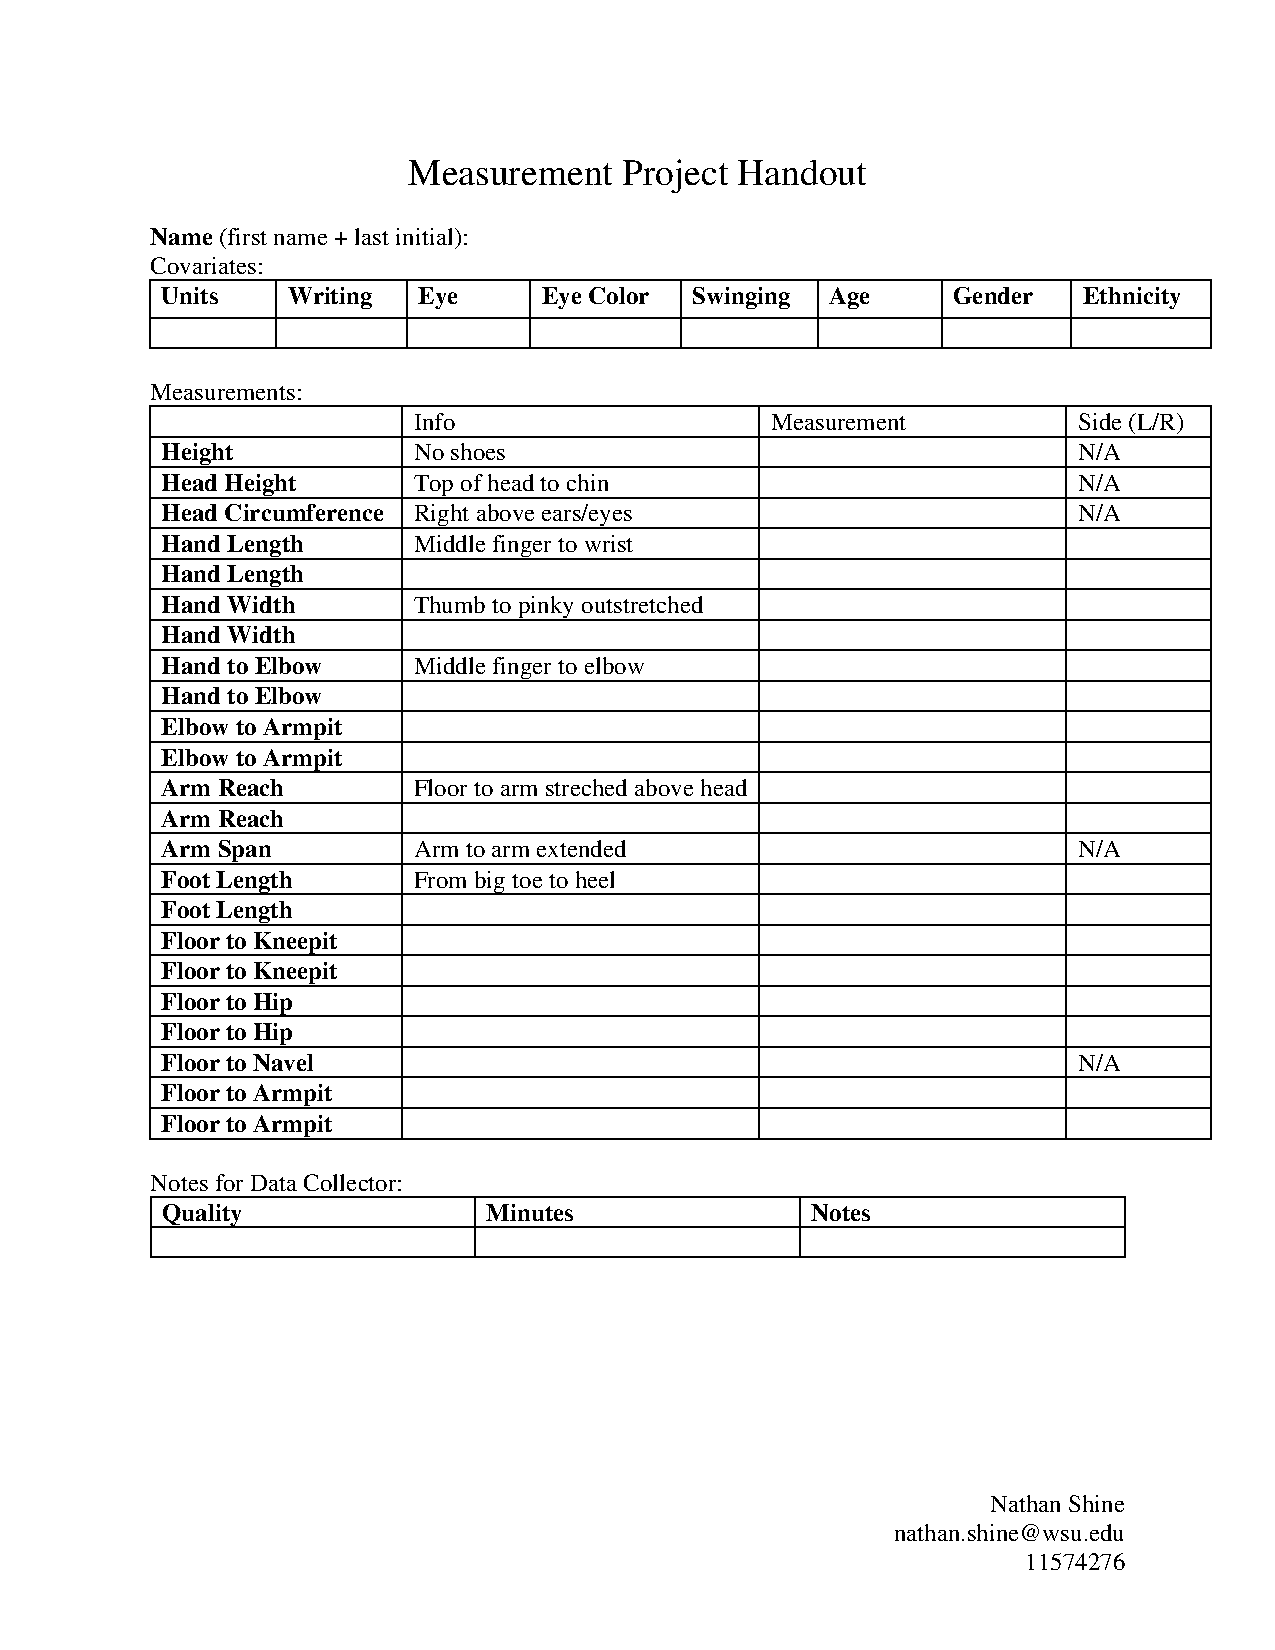
\includegraphics[trim = 0 0 0 0,clip,width=0.85\textwidth]{pdfs/shine_handout.pdf} }
    \end{center}
    \label{fig:handout-1}
    \hrule
\end{figure}

\newpage

\begin{figure}[!ht]
    \begin{subfigure}[h]{0.5\textwidth}
    \centering
    %  trim={<left> <lower> <right> <upper>}
    % https://shantoroy.com/latex/add-subfig-in-latex/
            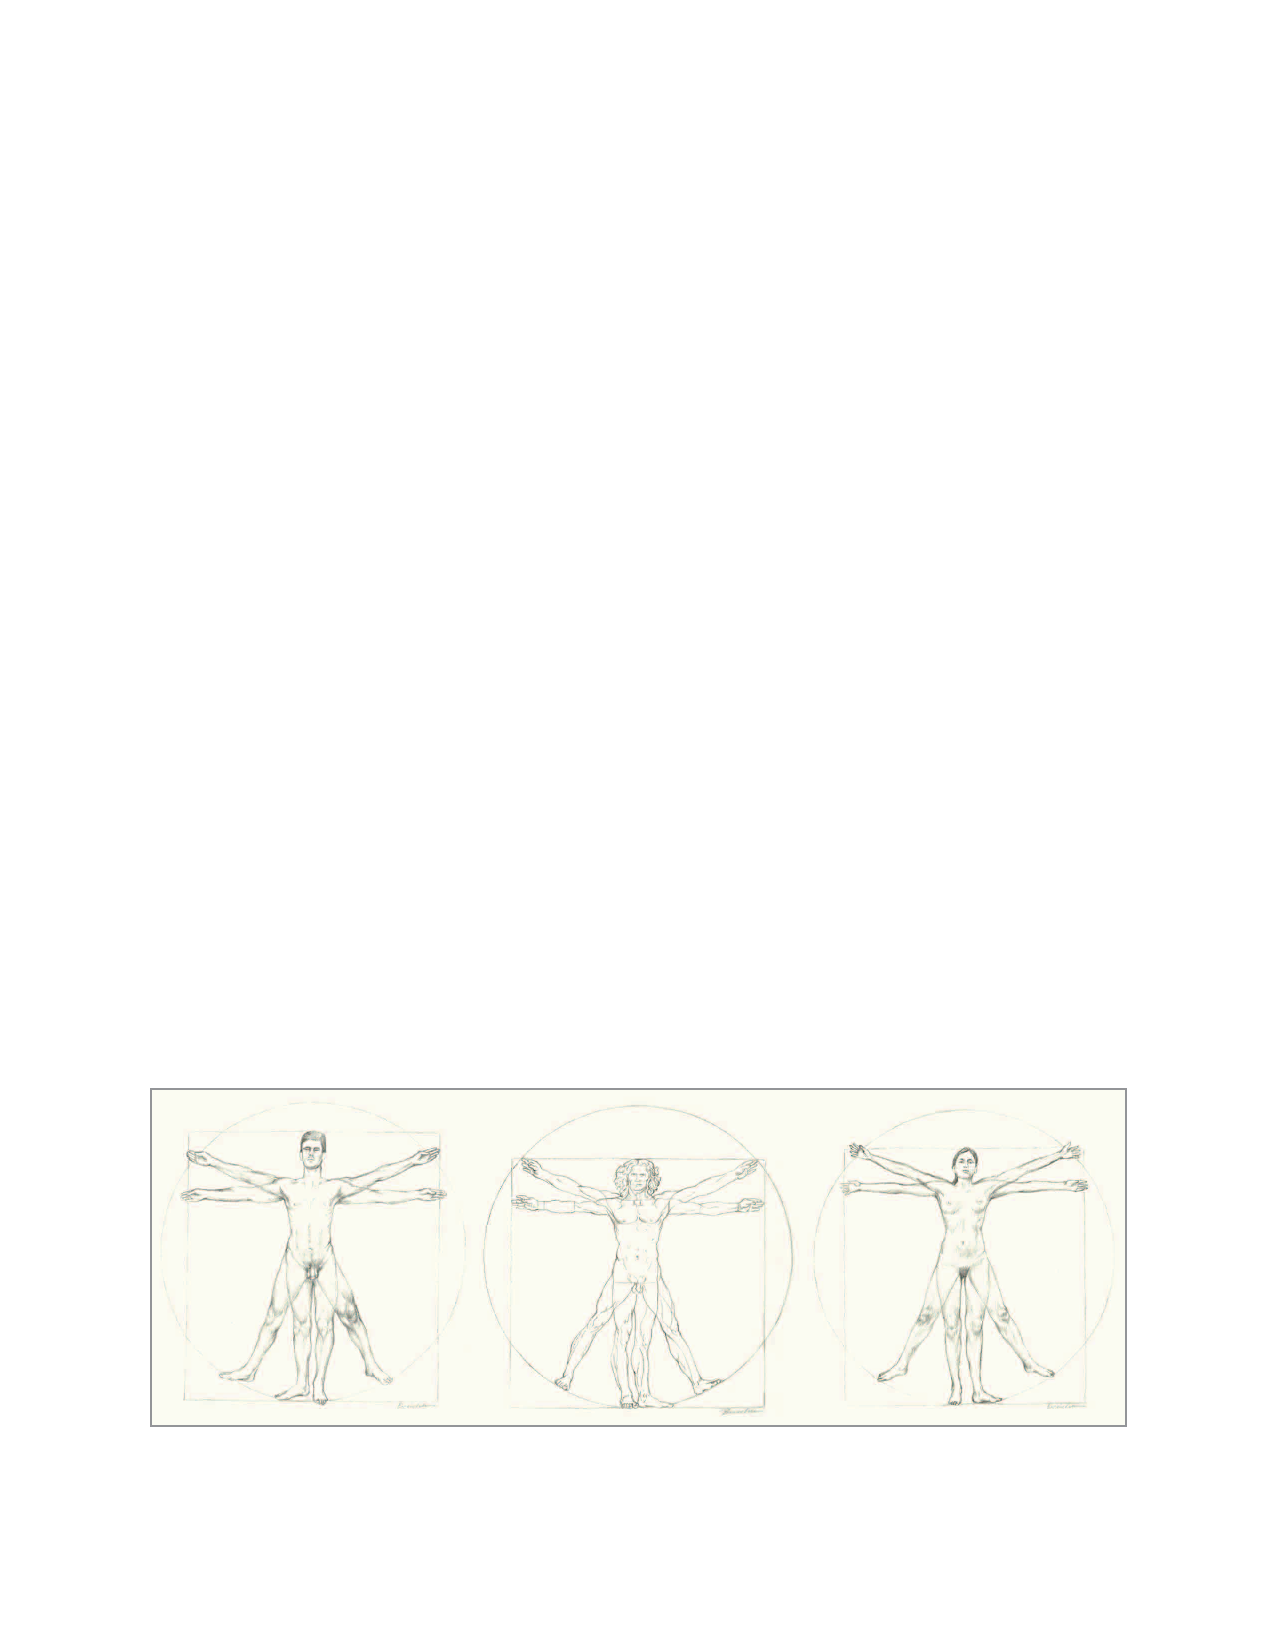
\includegraphics[trim = 0 0 11.25cm 0,clip,scale=1]{figures/Vitruvian.pdf}
        \caption{ \citet{Thomas:2020} discuss this. }
        \label{fig:sub-first}
    \end{subfigure}
    \begin{subfigure}[h]{0.5\textwidth}
    \centering
        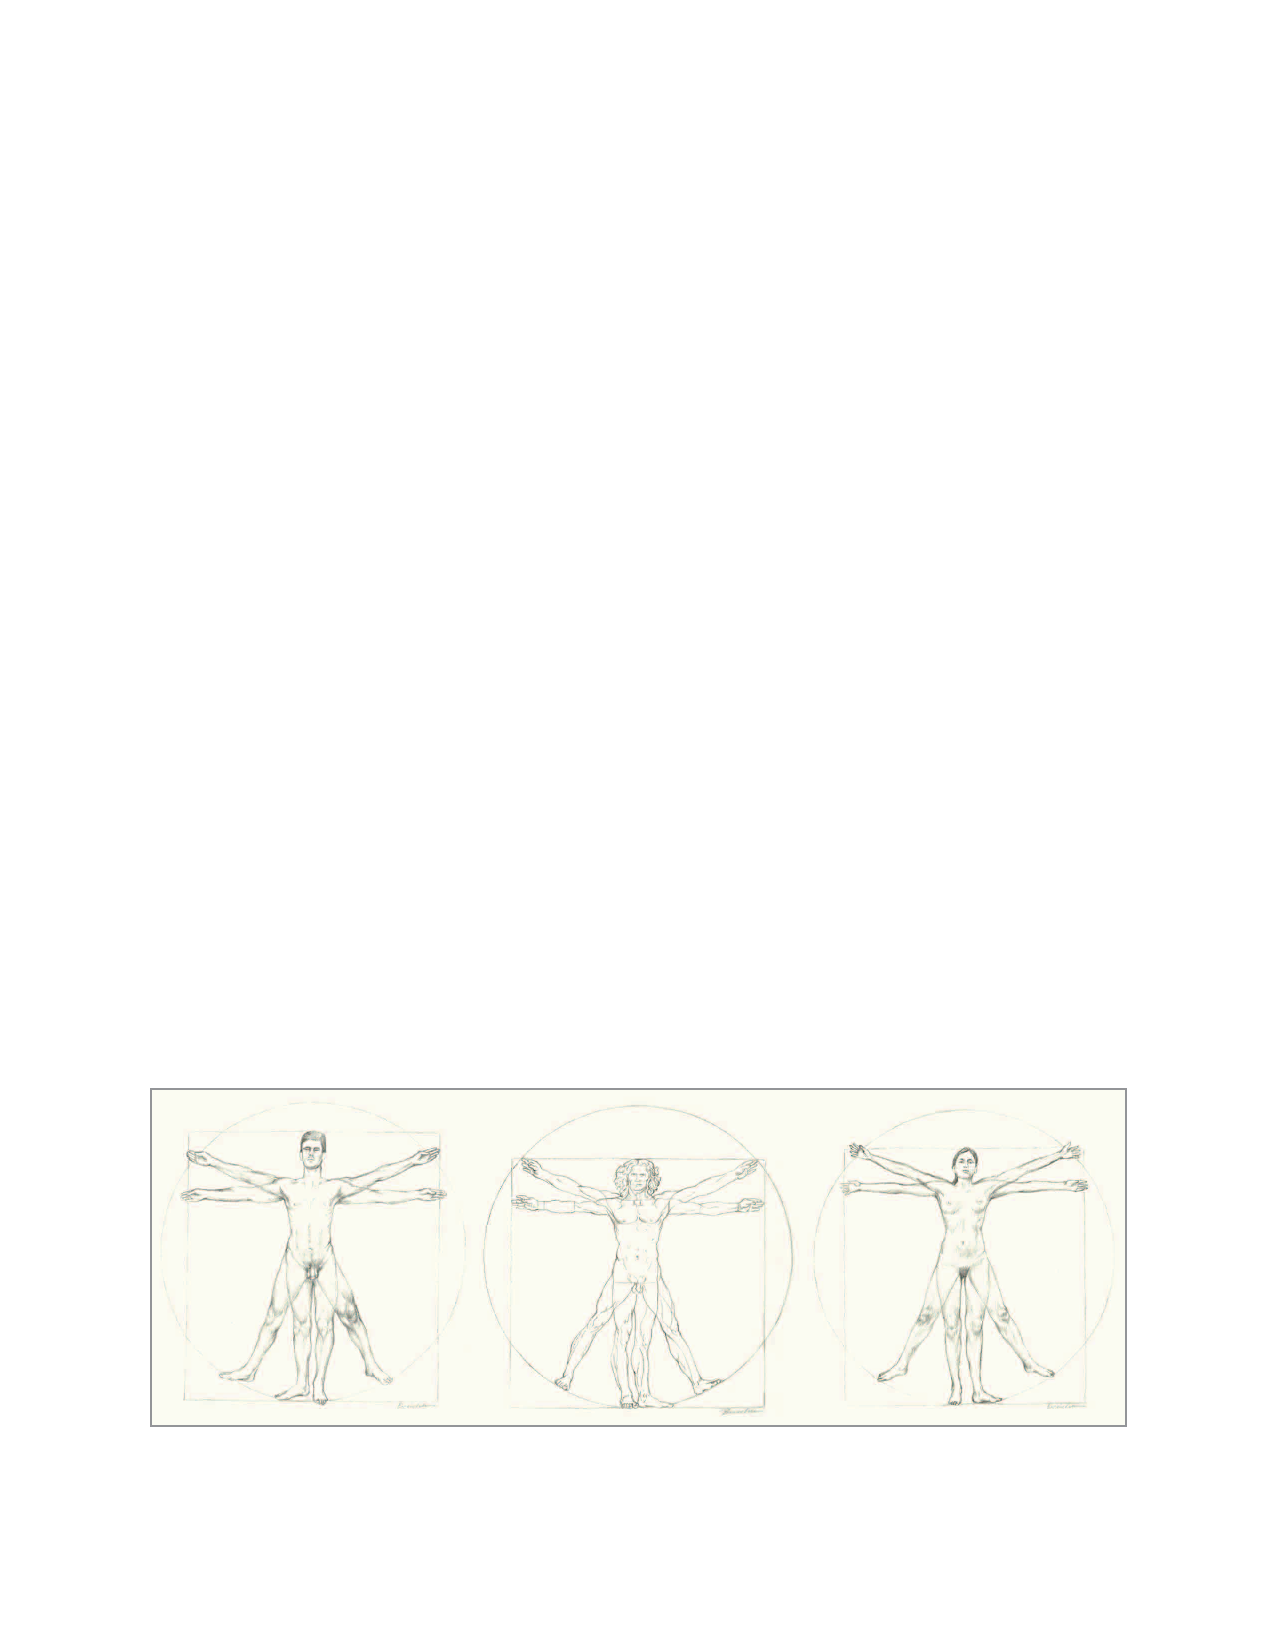
\includegraphics[trim = 11.25cm 0 0 0,clip,scale=1]{figures/Vitruvian.pdf}
            \caption{Schnitt realer Sensor \citep{Thomas:2020}}
        \label{fig:sub-second}
    \end{subfigure}
    \vspace{2.5mm}
    \hrule
    \vspace{2.5mm}
        \caption{\textbf{ Der Sensor in Theorie und Verwirklichung... caption at bottom instead? }  I can write a really long caption if I want. \newline This is using "crop" to include one image and trim it to appear as two.  Likely you will have two separate images if you use this option, so you would set the trim parameters all equal to 0.  \newline   This figure has subfigures which each also have a possible caption.   }
        \label{fig:combined}
    \vspace{-2.5mm}
    \hrule
\end{figure}

\newpage

\subsection{Preparing the Report Workspace as a subsection}
\label{sec:appendix-setup}

\subsubsection{Preparing the Report Workspace as a subsubsection}
\label{sec:appendix-setup2}

\paragraph{Preparing the Report Workspace as a paragraph}
\label{sec:appendix-setup3}

\subparagraph{Preparing the Report Workspace as a subparagrah}
\label{sec:appendix-setup4}

Below is the necessary functions and libraries required to run the code
referenced in this document.

\begin{Shaded}
\begin{Highlighting}[]
\KeywordTok{library}\NormalTok{(devtools);       }\CommentTok{\# required for source\_url}

\NormalTok{path.humanVerseWSU =}\StringTok{ "https://raw.githubusercontent.com/MonteShaffer/humanVerseWSU/"}
\KeywordTok{source\_url}\NormalTok{( }\KeywordTok{paste0}\NormalTok{(path.humanVerseWSU,}\StringTok{"master/misc/functions{-}project{-}measure.R"}\NormalTok{) );}
\end{Highlighting}
\end{Shaded}

\begin{verbatim}
## Warning: package 'Hmisc' was built under R version 4.0.3
\end{verbatim}

Below is the code to load the data and prepare it for analysis.

\begin{Shaded}
\begin{Highlighting}[]
\NormalTok{path.to.secret =}\StringTok{ "C:/Users/Nathan/Dropbox/\_\_student\_access\_\_/\_SECRET\_/"}\NormalTok{;}

\NormalTok{measure =}\StringTok{ }\NormalTok{utils}\OperatorTok{::}\KeywordTok{read.csv}\NormalTok{( }\KeywordTok{paste0}\NormalTok{(path.to.secret, }\StringTok{"measure{-}students.txt"}\NormalTok{), }\DataTypeTok{header=}\OtherTok{TRUE}\NormalTok{, }\DataTypeTok{quote=}\StringTok{""}\NormalTok{, }\DataTypeTok{sep=}\StringTok{"|"}\NormalTok{);}
\CommentTok{\#path.my.github = "https://raw.githubusercontent.com/nshine787/WSU\_STATS419\_FALL2020/";}
\CommentTok{\# source\_url(paste0(path.my.github, \textquotesingle{}master/functions/functions{-}project{-}measure.R\textquotesingle{}))}

\NormalTok{path.project =}\StringTok{ "C:/Users/Nathan/Documents/GitHub/WSU\_STATS419\_FALL2020/"}
\KeywordTok{source}\NormalTok{(}\KeywordTok{paste0}\NormalTok{(path.project, }\StringTok{\textquotesingle{}functions/functions{-}project{-}measure.R\textquotesingle{}}\NormalTok{))}

\CommentTok{\# this is your function}
\CommentTok{\# put in the same "units"}
\CommentTok{\# merge left/right}
\CommentTok{\# build proportion data}
\CommentTok{\# and so on ... }
\CommentTok{\# relevantColumns = c(\textquotesingle{}height\textquotesingle{}, )}
\NormalTok{relevantColumns =}\StringTok{ }\KeywordTok{c}\NormalTok{(}\StringTok{\textquotesingle{}height\textquotesingle{}}\NormalTok{, }\StringTok{\textquotesingle{}head.height\textquotesingle{}}\NormalTok{,}\StringTok{\textquotesingle{}arm.span\textquotesingle{}}\NormalTok{,}\StringTok{\textquotesingle{}hand.length\textquotesingle{}}\NormalTok{,}\StringTok{\textquotesingle{}foot.length\textquotesingle{}}\NormalTok{,}\StringTok{\textquotesingle{}floor.kneepit\textquotesingle{}}\NormalTok{,}\StringTok{\textquotesingle{}shoulder.width\textquotesingle{}}\NormalTok{)}
\NormalTok{measure.df =}\StringTok{ }\KeywordTok{prepareMeasureData}\NormalTok{(measure);}
\end{Highlighting}
\end{Shaded}

\begin{verbatim}
## Warning: package 'measurements' was built under R version 4.0.3
\end{verbatim}

\begin{verbatim}
## Warning in `[<-.factor`(`*tmp*`, iseq, value = "nb"): invalid factor level, NA
## generated
\end{verbatim}

\begin{Shaded}
\begin{Highlighting}[]
\NormalTok{measure.males.df =}\StringTok{ }\KeywordTok{grabGenderRows}\NormalTok{(measure.df,}\StringTok{\textquotesingle{}m\textquotesingle{}}\NormalTok{)[,relevantColumns]}
\NormalTok{measure.females.df =}\StringTok{ }\KeywordTok{grabGenderRows}\NormalTok{(measure.df,}\StringTok{\textquotesingle{}f\textquotesingle{}}\NormalTok{)[,relevantColumns]}

\NormalTok{proportions.male =}\StringTok{ }\NormalTok{measure.males.df}\OperatorTok{/}\NormalTok{measure.males.df}\OperatorTok{$}\NormalTok{height}
\NormalTok{proportions.female =}\StringTok{ }\NormalTok{measure.females.df}\OperatorTok{/}\NormalTok{measure.females.df}\OperatorTok{$}\NormalTok{height}
\end{Highlighting}
\end{Shaded}

Below is the code to generate the summary statistics and save them as a
table that you see in Section \ref{sec:data-summary}.

\begin{Shaded}
\begin{Highlighting}[]
\KeywordTok{summary}\NormalTok{(measure.males.df)}
\end{Highlighting}
\end{Shaded}

\begin{verbatim}
##      height       head.height       arm.span      hand.length   
##  Min.   :137.0   Min.   :17.78   Min.   :139.0   Min.   :15.00  
##  1st Qu.:172.0   1st Qu.:21.59   1st Qu.:169.5   1st Qu.:18.30  
##  Median :177.8   Median :23.00   Median :177.8   Median :19.05  
##  Mean   :176.4   Mean   :22.98   Mean   :178.3   Mean   :19.15  
##  3rd Qu.:182.7   3rd Qu.:24.00   3rd Qu.:185.2   3rd Qu.:20.00  
##  Max.   :191.1   Max.   :29.50   Max.   :224.0   Max.   :24.00  
##  NA's   :8       NA's   :7       NA's   :8       NA's   :4      
##   foot.length    floor.kneepit   shoulder.width 
##  Min.   :20.00   Min.   :38.00   Min.   : 1.50  
##  1st Qu.:25.09   1st Qu.:44.77   1st Qu.:23.81  
##  Median :26.02   Median :47.00   Median :36.00  
##  Mean   :26.15   Mean   :47.23   Mean   :35.80  
##  3rd Qu.:27.59   3rd Qu.:50.00   3rd Qu.:44.00  
##  Max.   :30.50   Max.   :58.00   Max.   :92.00  
##  NA's   :9       NA's   :10      NA's   :18
\end{verbatim}

\begin{Shaded}
\begin{Highlighting}[]
\KeywordTok{summary}\NormalTok{(measure.females.df)}
\end{Highlighting}
\end{Shaded}

\begin{verbatim}
##      height       head.height       arm.span      hand.length   
##  Min.   :140.0   Min.   :17.50   Min.   :141.7   Min.   :13.97  
##  1st Qu.:158.0   1st Qu.:20.31   1st Qu.:157.2   1st Qu.:16.80  
##  Median :162.6   Median :21.50   Median :163.0   Median :17.35  
##  Mean   :162.5   Mean   :21.75   Mean   :164.1   Mean   :17.57  
##  3rd Qu.:167.7   3rd Qu.:22.86   3rd Qu.:171.4   3rd Qu.:18.38  
##  Max.   :181.0   Max.   :33.02   Max.   :198.5   Max.   :21.20  
##  NA's   :8       NA's   :7       NA's   :9       NA's   :3      
##   foot.length    floor.kneepit   shoulder.width 
##  Min.   :13.50   Min.   :34.92   Min.   : 1.70  
##  1st Qu.:22.54   1st Qu.:41.00   1st Qu.:22.00  
##  Median :23.50   Median :43.00   Median :31.11  
##  Mean   :23.62   Mean   :43.49   Mean   :30.28  
##  3rd Qu.:24.40   3rd Qu.:45.72   3rd Qu.:36.83  
##  Max.   :27.50   Max.   :52.38   Max.   :61.50  
##  NA's   :13      NA's   :13      NA's   :13
\end{verbatim}




%% appendices go here!


\newpage
\theendnotes

%%%%%%%%%%%%%%%%%%%%%%%%%%%%%%%%%%%  biblio %%%%%%%%
\newpage
\begin{auxmulticols}{2}
\singlespacing 
\bibliography{./../biblio/master.bib}

%%%%%%%%%%%%%%%%%%%%%%%%%%%%%%%%%%%  biblio %%%%%%%%
\end{auxmulticols}

\newpage
{
\hypersetup{linkcolor=black}
\setcounter{tocdepth}{3}
\tableofcontents
}



\end{document}